\section{Evaluation Setup}
    \begin{figure}
        \centering
        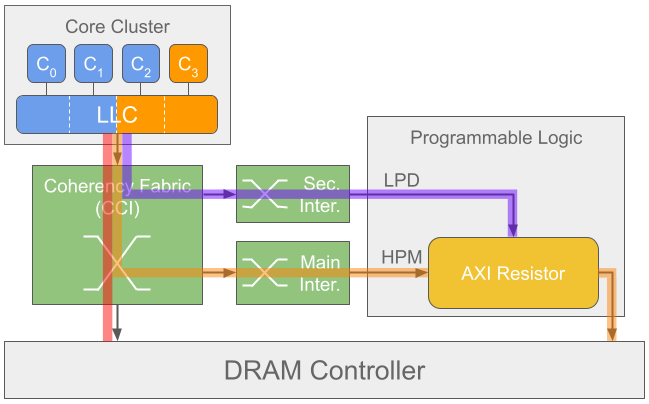
\includegraphics[scale=0.35]{images/Evaluation_setup.png}
        \caption{}
        \label{fig:system_schematic}
    \end{figure}
    For our experiment, we use the Xilinx ZCU102 develpment board \cite{Xilinx-ULTRASCALE-TRM}, a platform associating a tarditional Processing System (or PS) with a tightly integrated Programmable Logic (or PL). Figure \ref{fig:system_schematic} offers a schematic representation of the platform.
    The PS side features four ARM Cortex-A53 cores \cite{ARM-cortex-A53} connected altogether thanks to a shared last-level of cache of 1MB. These resources are shared between two actors: a \emph{victim} and a \emph{attacker}. On the other hand, the PL side is programmed with a custom IP\footnote{Intelectual Property} called AXI-Resistor (more details in section \ref{subsec:axi-resistor}). In a PLIM module fashion \cite{PLIM20}, the latter is connected to both the PS side and the DRAM controller thanks to the HPM and the HP ports respectivelly. The AXI-Resistor will be used as the slow memory target.

    In the present scenario, the victim executes a set of tasks addressing directly the main memory (i.e. the path highlited in red in Figure \ref{fig:system_schematic}), whereas the attacker targets the AXI-Resistor with read transactions.\\

    This section presents the technical details of the different components and actors of the experiments. Further details regarding the organization of the PS side are given in section \ref{subsec:processing_system_organization}. In section \ref{subsec:attacker_reading_memory_bomb}, a description of the attacker is given. Finally, a complete description of the AXI-Resistor is given section \ref{subsec:axi-resistor}.

    \subsection{Processing System Organization}
        \label{subsec:processing_system_organization}
        As previously mentioned, the PS side and especially the core cluster is shared by both the victim and the attacker. The actors are assigned to different cores via the Jailhouse hypervisor\cite{jailhouse}. Doing so, each actor is an independent \emph{virtual machine} (or VM), ensuring that the observed delays cannot be imputed to common software stack. In addition, the cache coloring feature of Jailhouse has been used to partition the cache, preventing inter-core cache line evictions.

        The victim virtual machine is a full-fledged Linux system tasked to run a given payload. In this experiments, the payload is issued from the San-Diego Vision Benchmark Suite \cite{SD-VBS}. As illustrated in the Figure \ref{fig:system_schematic} (colored in blue), this virtual machine is allocated three cores and half of the last level of cache (or LLC).

        The attacker virtual machine is a lightweight baremetal application in charge of emitting sequential read transactions toward the desired target. As shown by the Figure \ref{fig:system_schematic}, the attacker runs on one core and is allocated two quarters of the last level of cache. The first quarter allows the attacker to access the main memory where its code is located (via the path highlighted in red in Figure \ref{fig:system_schematic}) and the second quarter is dedicated to the data read from AXI-Resistor (the orange path in Figure \ref{fig:system_schematic}). Isolating the two address space is important as it enables us to have a control over the amount of transactions targetting the AXI-Resistor.

        Globally, the two virtual machines are perfectly isolated. The only exception being that the attacker also access the main memory to load its code. Nonetheless, this should introduce little or no inter-core interference.

    \subsection{Attacker - Reading Memory Bomb}
        \label{subsec:attacker_reading_memory_bomb}
        The design of the attacker (i.e. the read memory bomb) must be thought carefully, even with the aforementioned precautions. In fact, let alone a read memory bomb will steadily fetch data and will fill its last level of cache partition. At one point, one of these fetches will provoke a cache line eviction. If not under control, these cache line evictions will generate write back transaction that will accumulate in the MSHR, potentially leading to the phenomenon reported by \cite{Heechul_DDOS_attacks_on_shared_cache}.


        \begin{lstlisting}[language=C, caption={Read memory-bomb code}, label={lst:bomb_listing}, basicstyle=\small, captionpos=b]
void do_reads(void) {
    crc = 0;
    for (int i = 0; i < size; i += LINE_SIZE) {
        crc += buffer[i];
        __dsb(SY);
    }
}
        \end{lstlisting}

        This side effect can only be avoided by throttling down the attacker core. We enforce this by following each read request by a \emph{Data Synchronisation Barrier} (or \texttt{DSB}) as shown in Listing \ref{lst:bomb_listing}. Doing so ensures that at most, only one read transaction toward the AXI-Resistor will be emited at a time. Subsequently, it guarantees that there is never more than one write back transaction linked to the attacker in the MSHR.

    \subsection{AXI-Resistor IP}
        \label{subsec:axi-resistor}
        \begin{figure}
            \centering
            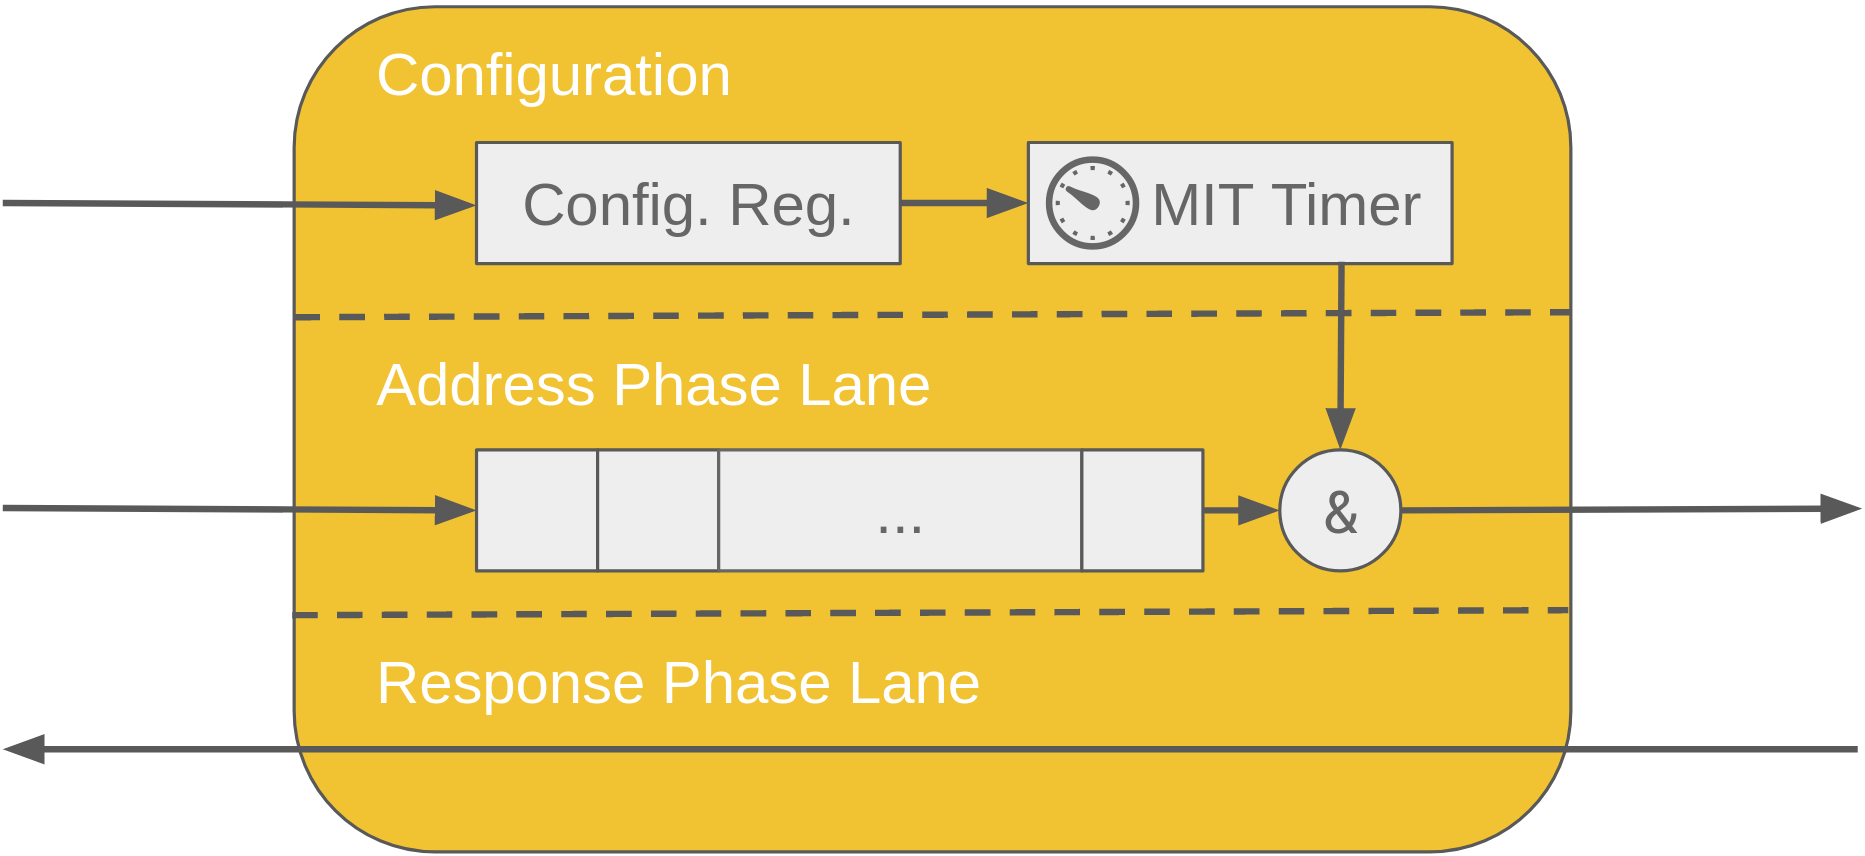
\includegraphics[scale=0.11]{images/AXI-Resistor.png}
            \caption{}
            \label{fig:axi_resistor}
        \end{figure}

        The AXI-resistor IP is a PLIM module \cite{PLIM20}, meaning that it is a module located on the PL side that sits between the core cluster and the DRAM controller. By targeting, the HPM port adddress space, the cores indirectly access the main memory as transactions received by a PLIM module are redirected toward the DRAM controller.  For our experiment, the AXI-Resistor is used as a slow cacheable memory target.

        Architecturally, the AXI-Resistor is simply composed of a queue buffering the the address phases of the incomming AXI transactions \cite{ARM-AXI} (the response phase is not intercepted) and a timer releasing the address phase stored in the head of the queue with a given minimun inter-arrival period (or MIT). The MIT is expressed in clock cycles (or CC) and the PL side runs at 250MHz. Thanks to a configuration port accessible via the purple path in Figure \ref{fig:system_schematic}, the MIT can be reprogrammed at run-time.

        Because each the address phase of each transaction is intercepted by the the AXI-Resistor before arriving to the DRAM controller, the latter is unaware of the transaction and no internal mechanism is activated.
